\documentclass[a4paper,12pt,twocolumn]{article}

\usepackage[papersize={216mm,330mm},tmargin=15mm,bmargin=15mm,lmargin=15mm,rmargin=15mm]{geometry}
\usepackage[english]{babel}
\usepackage[utf8]{inputenc}
\usepackage{amsmath,amssymb}% for \eqref
\usepackage{graphicx}
\usepackage[colorinlistoftodos]{todonotes}
\pagestyle{myheadings}
\markright{Business Intelligence vs Business Analytics}

\title{Business Intelligence vs Business Analytics}
\date{\today}
\begin{document}
\maketitle
\subsubsection*{Abstract}
In recent years, organizations have increasingly turned to advanced software
solutions to manage workloads, maintain protability and ensure competitiveness
within their respective industries. While there are several options available, business
intelligence tools (BI) and business analytics tools (BA) are arguably the most
widely implemented data management solutions. Business analysts and software
buyers alike often ask what are the key diferences between business intelligence vs business analytics.
\subsubsection*{Resumén}
En los últimos años, las organizaciones han recurrido cada vez mas a soluciones de software
avanzadas para administrar las cargas de trabajo, mantener la rentabilidad y asegurar la
competitividad dentro de sus respectivas industrias. Si bien hay varias opciones disponibles,
las herramientas de inteligencia de negocios (BI) y las herramientas de análisis de negocios
(BA) son posiblemente las soluciones de administración de datos mas implementadas. Los
analistas de negocios y los compradores de software a menudo preguntan cuales son las diferencias
clave entre la inteligencia de negocios y los análisis de negocios.
\subsubsection*{Introducci\'on}
Las soluciones de inteligencia empresarial se encuentran entre las herramientas
de administración de datos mas valiosas disponibles. Las soluciones de BI recopilan
y analizan datos actuales y procesables con el n de proporcionar información para
mejorar las operaciones comerciales. ¿Esta buscando formas de entender mejor sus
operaciones comerciales? ¿Que hay de descubrir puntos de dolor en sus flujos de
trabajo? ¿Que hay de analizar grandes conjuntos de datos para obtener información
valiosa? Necesita una solución de inteligencia de negocios.
\begin{center}
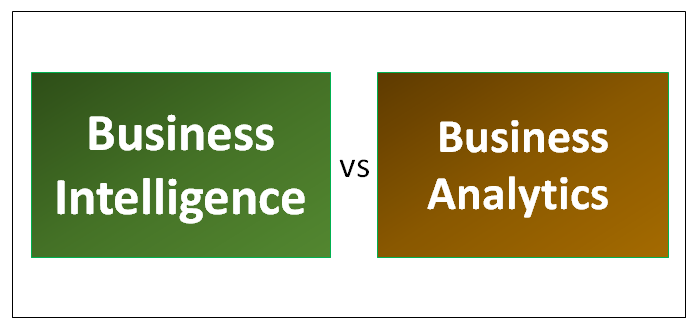
\includegraphics[width=8cm]{./Imagenes/bivsba}
\end{center}

\section*{1.MARCO TEÓRICO} 

\textbf {1.1 INTELIGENCIA DE NEGOCIOS}\\
La inteligencia de negocios se define como la habilidad corporativa para tomar decisiones. Esto se logra mediante el uso de metodologías, aplicaciones y tecnologías que permiten reunir, depurar, transformar datos, y aplicar en ellos técnicas analíticas de extracción de conocimiento (\footnote{Parr 2000}), los datos pueden ser estructurados para que indiquen las características de un área de interés (\footnote{Stackowiak et al. 2007}), generando el conocimiento sobre los problemas y oportunidades del negocio para que pueden ser corregidos y aprovechados respectivamente.(\footnote{Ballard et al. 2006})

Implementar herramientas de BI dentro de la organización permite soportar las decisiones que se toman; al nivel interno ayuda en la gestión del personal (\footnote{Sharma et al. 2009}) y del lado externo produce ventajas sobre sus competidores (\footnote{Maureen 2009}). Existen ocasiones en las cuales no se pueden lograr todos los beneficios que tiene BI; debido al proceso que lleva consigo implementar un proyecto de estas características, se puede cometer errores en la definición del planteamiento de las necesidades de conocimiento de la empresa; el no determinar la magnitud de los problemas de información a solucionar generalmente repercute en el fracaso del proyecto.


Agile BI Governance establece 4 valores básicos, pero dependiendo de cada organización puede incluir los que vayan en relación con su propia estrategia. 
\item • \textbf{Adaptabilidad Continúa.} La incertidumbre y el cambio continuo son el estado natural de los sistemas de toma de decisiones, pero parece ser que muchas organizaciones aún no son conscientes de ellos. En este tipo de proyectos siempre se está cambiando el punto de vista analítico. 
\item • \textbf{Trabajo Conjunto.}  El usuario operativo del software ha de ser parte activa dentro de los grupos de IT que desarrollan los sistemas de BI.
\item • \textbf{Jerarquías Flexibles.} Los grupos de trabajo dentro del Agile BI Governance deberán estar estructurados con jerarquías flexibles que fomenten el intercambio de información.
\item • \textbf{Personas Antes que Procesos.}  Priorizar la entrega de la información a las personas que controlan los procesos y no tanto en definir los procesos que han de controlar las personas. (\footnote{Fernández 2008})
\textbf{}\\
\textbf{}\\
\textbf {1.2 DATA WAREHOUSE}\\

Es el proceso de extraer datos de distintas aplicaciones (internas y externas), para que una vez depurados y especialmente estructurados sean almacenados en un depósito de datos consolidado para el análisis del negocio. Requiere una combinación de metodologías, técnicas, hardware y los componentes de software que proporcionan en conjunto la infraestructura para soportar el proceso de información (\footnote{Stackowiak et al. 2007}). La estructura que se defina debe reflejar las necesidades y características del negocio, sus departamentos, equipos de trabajo y directivos1 , esto permitirá responder a interrogantes generados al tratar de tomar las decisiones (\footnote{Witten 2000}) y con el tiempo se va convirtiendo en la memoria corporativa (\footnote{Wang 2009}); describiendo el pasado y el presente de la empresa. Data Warehouse desglosa, resume, ordena y compara, pero no descubre, ni predice. (\footnote{Flores 2004}) 

\textbf{}\\
Para la construcción de un Data Warehouse se establecen tres etapas; la primera está dedicada a examinar el esquema Entidad Relación de la base de datos operacional, generando los esquemas multidimensionales candidatos. 

\textbf{}\\
La segunda etapa, consiste en recoger los requisitos de usuario por medio de entrevistas, para obtener información acerca de las necesidades de análisis de estos, y la tercera etapa, contrasta la información obtenida en la segunda etapa, con los esquemas multidimensional candidatos formados en la primera etapa generando así, una solución que refleja los requisitos de usuario (\footnote{Zenaido 2008}). 

\textbf{}\\
Por otra parte implementar una solución de este tipo, ocasiona un costo que no todas las organizaciones están dispuestas a pagar (debido a sus capacidades de inversión), es por eso que los promotores del proyecto dentro de la empresa deben persuadir a los directivos y compañeros de trabajo, una buena alternativa de hacerlo es mediante el uso de técnicas administrativas, que permitan conocer a los directivos como se puede establecer el retorno de la inversión del proyecto equiparando inversión contra beneficios.  (\footnote{Arturo 2001})

\textbf{}\\
Al ser un depósito de datos consolidado para el análisis del negocio necesita tomar datos de distintas fuentes, Internas y Externas (\footnote{Stackowiak et al. 2007}), y como las características de las empresas son diferentes la cantidad de registros almacenados en algunas de ellas puede llegar a ser de proporciones exponenciales; es por esta razón que se necesita de procesos que optimicen los tiempos de extracción, transformación y transferencia de los datos del sistemas de información a la fuente de datos esto se logra implementando técnicas incrementales que mediante el uso de Snapshots y Triggers, se encarguen de sacar, transformar y transferir los registros que existen en el sistema de información a la fuente de datos. (\footnote{Flores 2003})
\textbf{}\\

El uso de Data Warehouse es tan amplio que llega a diferentes tipos de organizaciones y distintos temas de interés, puede ser implementado con conceptos Administrativos, en la administración; ayuda en la identificación de elementos de cambio que definan una nueva manera de hacer negocios, en donde la competencia debe estar orientada a trabajar no sólo de forma aislada, sino en colaboración con los diversos grupos de interés o actores de la industria, buscando referencias diferenciadoras para alcanzar el éxito (\footnote{Romero 2002}), en empresas petroquímicas; incrementa la exactitud y precisión en la toma de decisiones con un 93.9\% en la rentabilidad (\footnote{Silva 2009}), en la Web; optimiza búsqueda Web de metadatos con características semi-inteligentes y también suministra el soporte necesario para crear comunidades de colaboración científica (\footnote{Luna et al. 2008 and Ameur et al. 2006}), en transformadores de potencia; almacenando, la monitorización del estado del flujo de energía (\footnote{Mariño et al. 2004}).
\textbf{}\\
\textbf{}\\
\textbf{1.3 OLAP}\\
El procesamiento analítico en línea permite obtener acceso a datos organizados y agregados de orígenes de datos empresariales2 , organiza subconjuntos de datos con una estructura multidimensional de manera que represente un significado especial o responda a una pregunta en particular 3 4 . (\footnote{Roussel 2006}) Estas herramientas soportan el análisis interactivo de la información de resumen, soportando muchas tareas de agrupación de datos que no pueden realizarse empleando las facilidades básicas de agregación y agrupamiento (\footnote{Silberschatz et al. 2006})
\textbf{}\\
\textbf{}\\
\textbf{1.3.1 TIPOS DE SISTEMAS OLAP}\\
Tradicionalmente, este sistema se clasifica según las siguientes categorías: 
\item • \textbf{ROLAP.} Implementación que almacena los datos en un motor relacional. Típicamente, los datos son detallados, evitando las agregaciones y las tablas se encuentran normalizadas.
\item • \textbf{MOLAP.} Esta implementación almacena los datos en una base de datos multidimensional. Para optimizar los tiempos de respuesta, el resumen de la información es usualmente calculado por adelantado. 
\item • \textbf{ HOLAP(Hybrid OLAP).} Almacena algunos datos en un motor relacional y otros en una base de datos multidimensional5 .
\textbf{}\\
Al igual que Data Warehouse, OLAP también es aplicable a un amplio rango de temas diferentes, uno de ellos es en Bases de Datos espaciales proporcionando características necesarias para los sistemas de tipo geográfico; como hechos, dimensiones, miembros, niveles, jerarquías, operaciones de navegación, operaciones de consolidación y comportamiento del clima (\footnote{Abril 2007 and Bernier et al. 2009}). También se utiliza el almacenamiento MOLAP y ROLAP, para generar índices que mejoran los tiempos de accesos a las consultas de manera que los tiempos de entrega de la información demore el menor tiempo posible (\footnote{Tamayo 2006}). Otra de las aplicaciones es en la educación al ser aplicado en ambientes de aprendizaje proporcionando las dimensiones y los indicadores necesarios para hacer la definición de un modelo de evaluación académica (\footnote{Cockbaine 2004}).
\textbf{}\\
\textbf{}\\
\textbf{1.4 CUADRO DE MANDO INTEGRAL}\\
El cuadro de mando integral (Balanced Scorecard) es una herramienta que permite alinear los objetivos de las diferentes áreas o unidades con la estrategia de la empresa y seguir su evolución6. El uso que se le puede dar a un Cuadro de Mando Integral es tan diverso que se puede contemplar autoevaluaciones del personal (Martínez 2008), hasta la definición de conceptos netamente organizacionales como son; la misión, la política de calidad; plan de comunicación, imagen corporativa, acciones de formación, catálogo de servicios; la confección de una cartera de clientes y la realización de acciones para conocer mejor sus opiniones y preferencias, así como para personalizar la presentación de la oferta de servicios para los clientes más importantes (Villalbía et al. 2005) (Matilla 2007). En fin, la ejecución de un cuadro de mando es tan amplia y generosa que puede llegar a cambiar la forma en que se presta un servicio en entidades públicas (Peters et al. 2007) (Weir et al. 2009).
\textbf{}\\
\textbf{}\\
\textbf{1.5 DATA MINING }
\textbf{}\\
Es el proceso de Seleccionar, Explorar, Modificar, Modelizar7 y valorar grandes cantidades de datos con el objetivo de descubrir conocimiento (Pérez 2006). El proceso debe ser automático o semi-automático. Los modelos hallados deben ser significativos demostrando cierto patrón o regla de comportamiento8 . Las aplicaciones más utilizadas son las que necesitan algún tipo de predicción. Por ejemplo, cuando una persona solicita una tarjeta de crédito, la compañía emisora quiere predecir si la persona, clasifica con el perfil identificado de usuarios morosos (Silberschatz et al. 2006). \textbf{}\\
\textbf{}\\
La minería de datos, permite la gestión en tiempo real de manera eficaz, es una herramienta aplicable a cualquier tipo de empresa. Una amplia gama de compañías puede tener aplicaciones exitosas con ella (Angeles et al. 2010). \textbf{}\\
\textbf{}\\
Beneficios asociados a la minería de datos (López 2004): Incremento de los resultados como consecuencia del aumento de la cuota de mercado; Fidelización de la clientela dada una mejor respuesta a sus requerimientos; Mejora del rendimiento; Reducción del factor riesgo; Optimización de las estrategias y toma de decisiones y Optimización de la gestión, maximizando rentabilidades. \textbf{}\\
\textbf{}\\
La aplicación de la Minería de Datos, además de permitir el descubrimiento del conocimiento en general, también se utiliza Biología soporta las investigaciones en la rama biológica, como herramienta insustituible para enfrentar la avalancha de datos que producen esta clase de proyectos (Febles 2002), en la Web Semántica; convierte la información en conocimiento que está distribuida en la web, proporcionando a las computadoras una mayor capacidad para gestionar y recuperar dichos datos (Rodríguez 2006), en las Redes de computadores; mediante la recolección de información acerca de los factores que impactan sobre la infraestructura de seguridad para descubrir la información relevante que ayude a tomar decisiones para corregir y/o mejorar las infraestructura de seguridad (Rojas 2005), en la Educación; haciendo seguimiento en los procesos de auto aprendizaje (Radenkovic et al. 2009).
\textbf{}\\
\textbf{}\\
\textbf{2.1 ANALISIS DE NEGOCIOS}
\textbf{}\\
El análisis de negocio(Business Analytics, BA) es el conjunto de métodos y técnicas utilizadas para trabajar como enlace entre los stackeholders, con el fin de comprender la estructura, políticas y operaciones de una organización y recomendar soluciones que permitan a la organización alcanzar sus objetivos (IIBA: International Institute of Business Analysis).\\
\textbf{}\\
El análisis de negocios implica la comprensión de cómo funcionan las organizaciones para llevar a cabo sus propósitos, y la definición de las capacidades que una organización requiere para proporcionar productos y servicios a los grupos de interés externos. Incluye la definición de los objetivos de la organización, cómo esos objetivos se conectan a objetivos específicos, que determinan las líneas de acción que una organización tiene que realizar para alcanzar esas metas y objetivos, y definir cómo las distintas unidades de organización y las partes interesadas dentro y fuera de esa organización interactúa.
\textbf{}\\
\begin{figure}[h!]
\centering
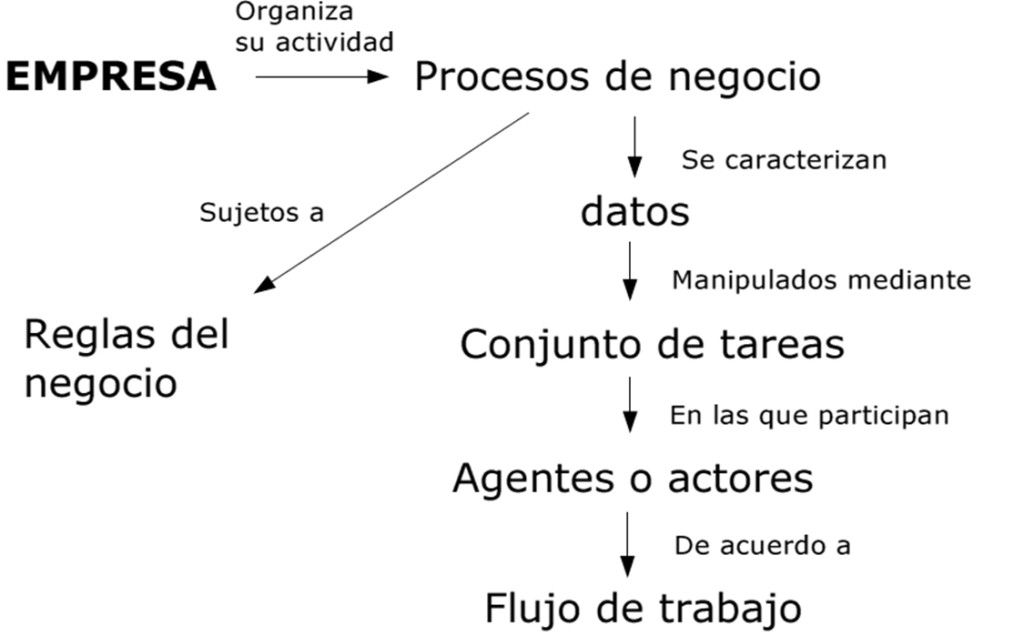
\includegraphics[width=8cm]{./Imagenes/anegocios}
\end{figure}
\textbf{2.2 Aplicaciones de Analisis de Negocios}\\
Las herramientas de inteligencia de negocio son aplicaciones digitales diseñadas para colaborar con el Business Intelligence durante el análisis y la presentación de datos.\\
La Inteligencia de Negocios o Business Intelligence (BI) permite a las compañías contar con la información adecuada para una mejor toma de decisiones.  Las compañías que implementan el BI logran sacar mayor provecho de las situaciones de crisis gracias a la posibilidad de contar con un análisis de mercado más acertado debido a que los datos pesados son transformados en importantes estrategias corporativas.
Actualmente, las herramientas de BI disponibles en el mercado son incontables, pero estas 20 no pueden pasar desapercibidas:
\textbf{}\\
\textbf{}\\
\textbf{}\\
\begin{center}
\begin{tabular}{|l|r|}\hline
\textbf{2.2.1} & \textbf{Microsoft Dynamics NAV}\\\hline
\textbf{2.2.2} & \textbf{Microsoft Dynamics CRM}\\\hline
\textbf{2.2.3} & \textbf{Oracle Business Intelligence}\\\hline
\textbf{2.2.4} & \textbf{Ultimus}\\\hline
\textbf{2.2.5} & \textbf{Office SharePoint Server}\\\hline
\textbf{2.2.6} & \textbf{QlikView}\\\hline
\textbf{2.2.7} & \textbf{Microsoft Performance Point Server}\\\hline
\textbf{2.2.8} & \textbf{Microsoft SQL Server}\\\hline
\textbf{2.2.9} & \textbf{JetReports}\\\hline
\textbf{2.2.10} & \textbf{Eclipse BIRT Projec}t\\\hline
\textbf{2.2.11} & \textbf{JasperReports}\\\hline
\textbf{2.2.12} & \textbf{LogiReport}\\\hline
\textbf{2.2.13} & \textbf{OpenI}\\\hline
\textbf{2.2.14} & \textbf{SPSS}\\\hline
\textbf{2.2.15} & \textbf{Pentaho}\\\hline
\textbf{2.2.16} & \textbf{RapidMiner}\\\hline
\textbf{2.2.17} & \textbf{Crystal Reports}\\\hline
\textbf{2.2.18} & \textbf{ApeSoft}\\\hline
\textbf{2.2.19} & \textbf{SAS Institute}\\\hline
\textbf{2.2.20} & \textbf{NiMbox}\\\hline
\end{tabular}
\end{center}

\begin{figure}[h!]
\centering
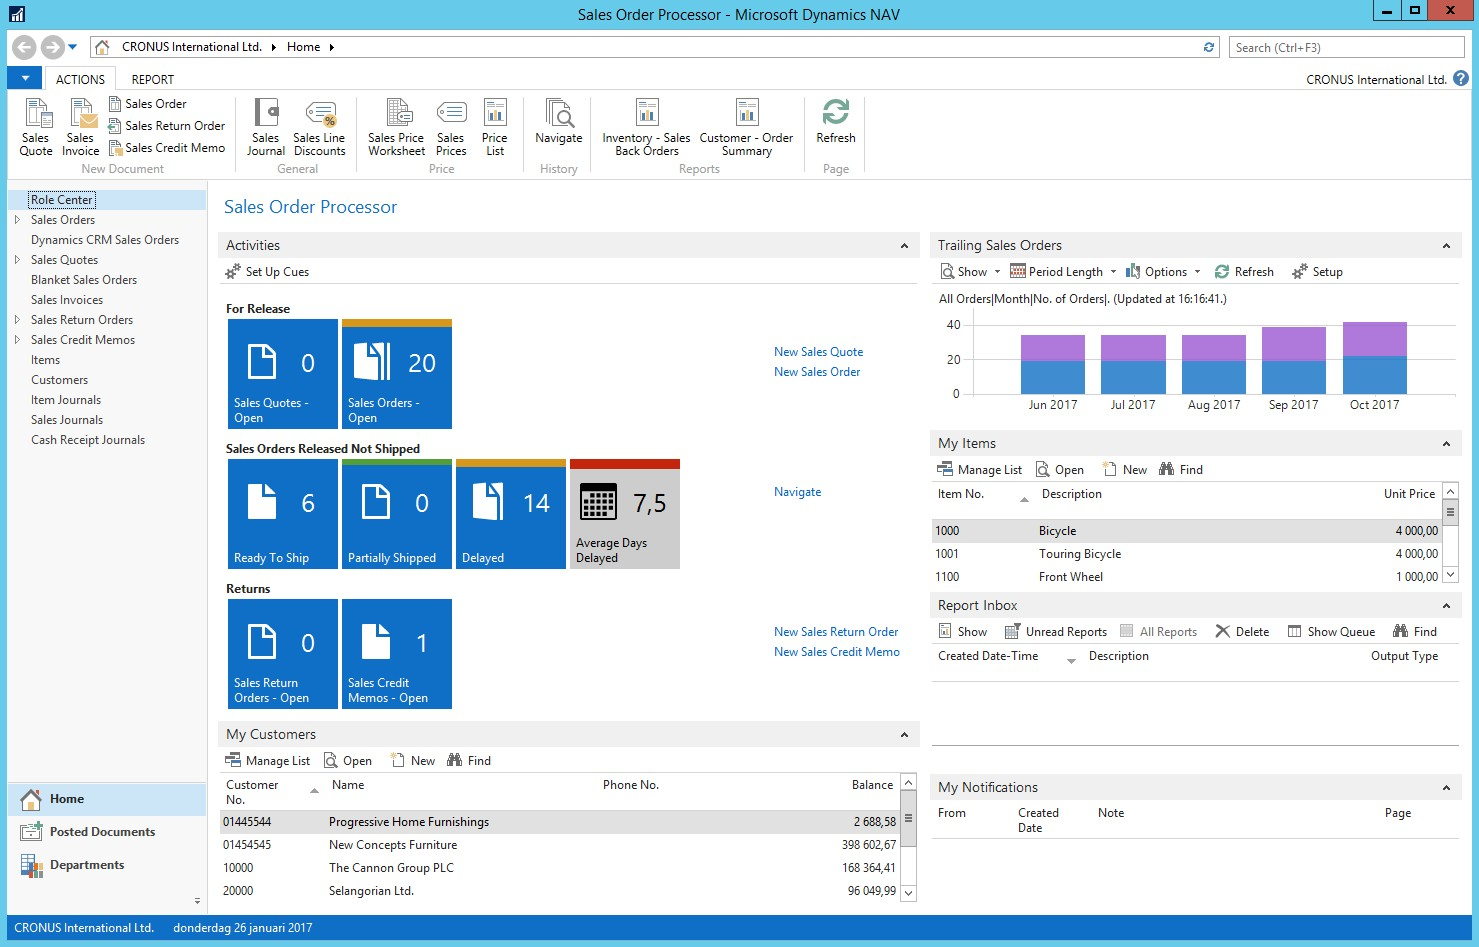
\includegraphics[width=9cm]{./Imagenes/BIimagen1}
\caption{\label{fig:01}Microsoft Dynamics NAV.(Especial para pequeñas y medianas empresas que buscan mejorar su competitividad)}
\end{figure}

\begin{figure}[h!]
\centering
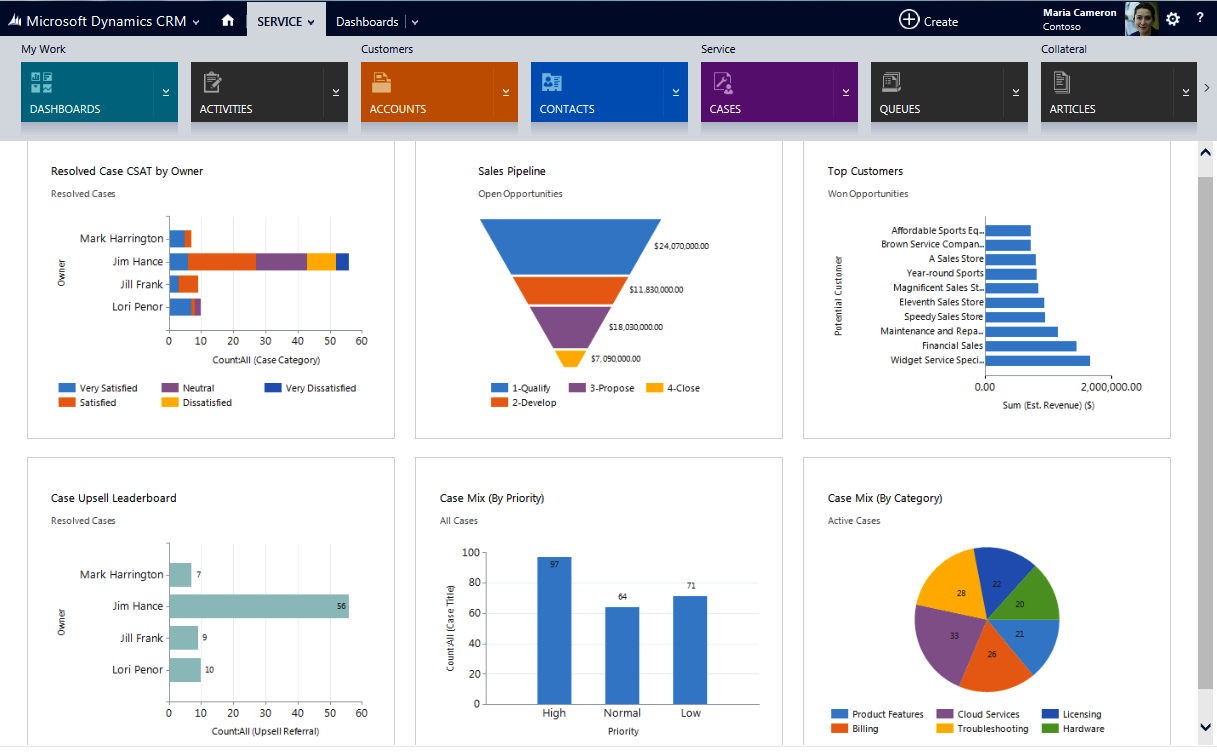
\includegraphics[width=9cm]{./Imagenes/BIimagen2}
\caption{\label{fig:01}Microsoft Dynamics CRM.(Efectiva para la administración de clientes.)}
\end{figure}
\textbf{}\\
\textbf{}\\
\textbf{}\\
\textbf{}\\
\begin{figure}[h!]
\centering
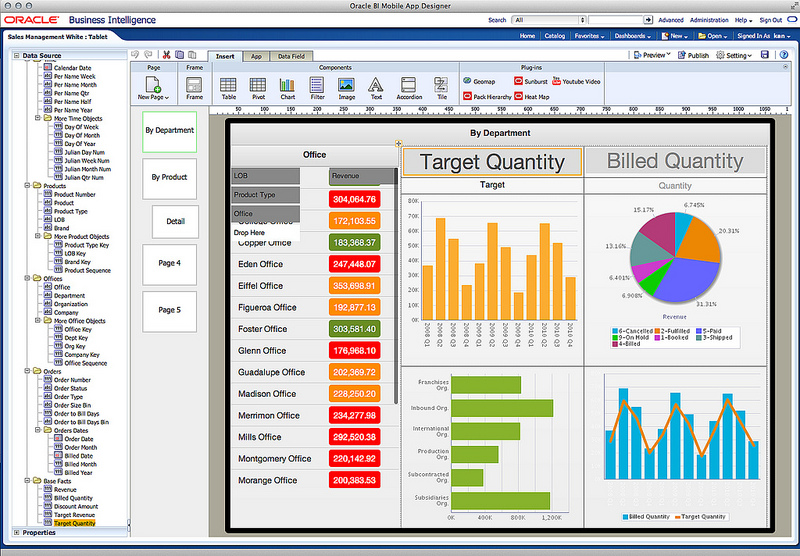
\includegraphics[width=8cm]{./Imagenes/BIimagen3}
\caption{\label{fig:01}Oracle Business Intelligence.(Una de las más completas en el mercado ya que cuenta con paneles interactivos, análisis predictivos en tiempo real, entre otros.)}
\end{figure}

\begin{figure}[h!]
\centering

\includegraphics[width=5cm]{./Imagenes/BIimagen4}
\caption{\label{fig:01}Ultimus.(Un entorno integrado que permite compartir información entre aplicaciones.)}
\end{figure}

\begin{figure}[h!]
\centering
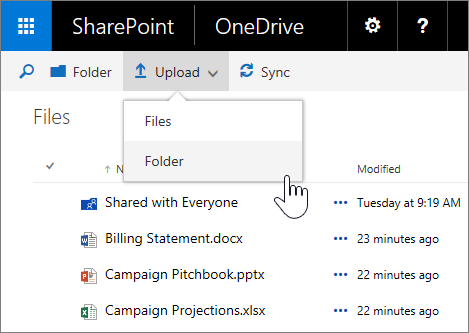
\includegraphics[width=8cm]{./Imagenes/BIimagen5}
\caption{\label{fig:01}Office SharePoint Server.(Facilita el acceso a la información en cualquier momento y lugar.Facilita el acceso a la información en cualquier momento y lugar.)}
\end{figure}

\begin{figure}[h!]
\centering
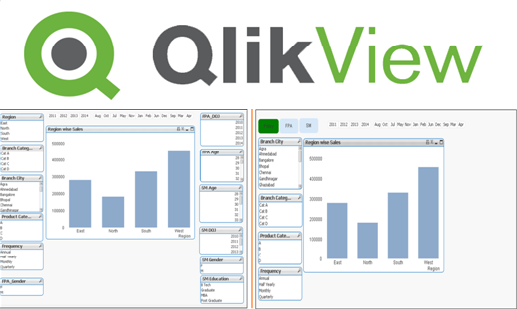
\includegraphics[width=8cm]{./Imagenes/BIimagen6}
\caption{\label{fig:01}QlikView.(Mantiene las bases de datos al alcance de una manera sin precedentes.)}
\end{figure}

\begin{figure}[h!]
\centering
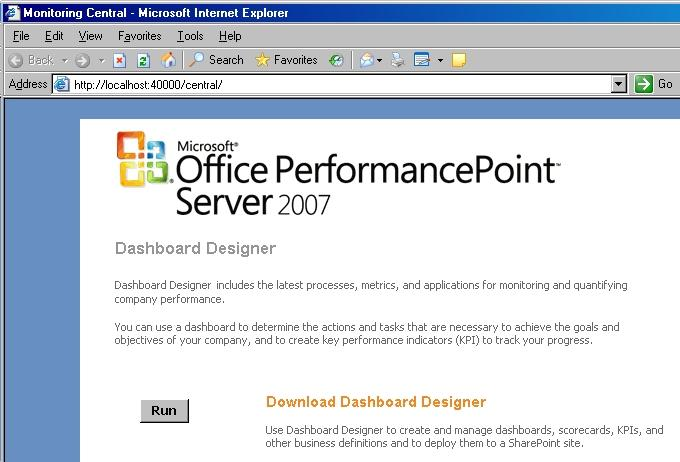
\includegraphics[width=9cm]{./Imagenes/BIimagen7}
\caption{\label{fig:01}Microsoft Performance Point Server.(Permite supervisar, alinear y hacer un plan de negocio.)}
\end{figure}

\begin{figure}[h!]
\centering
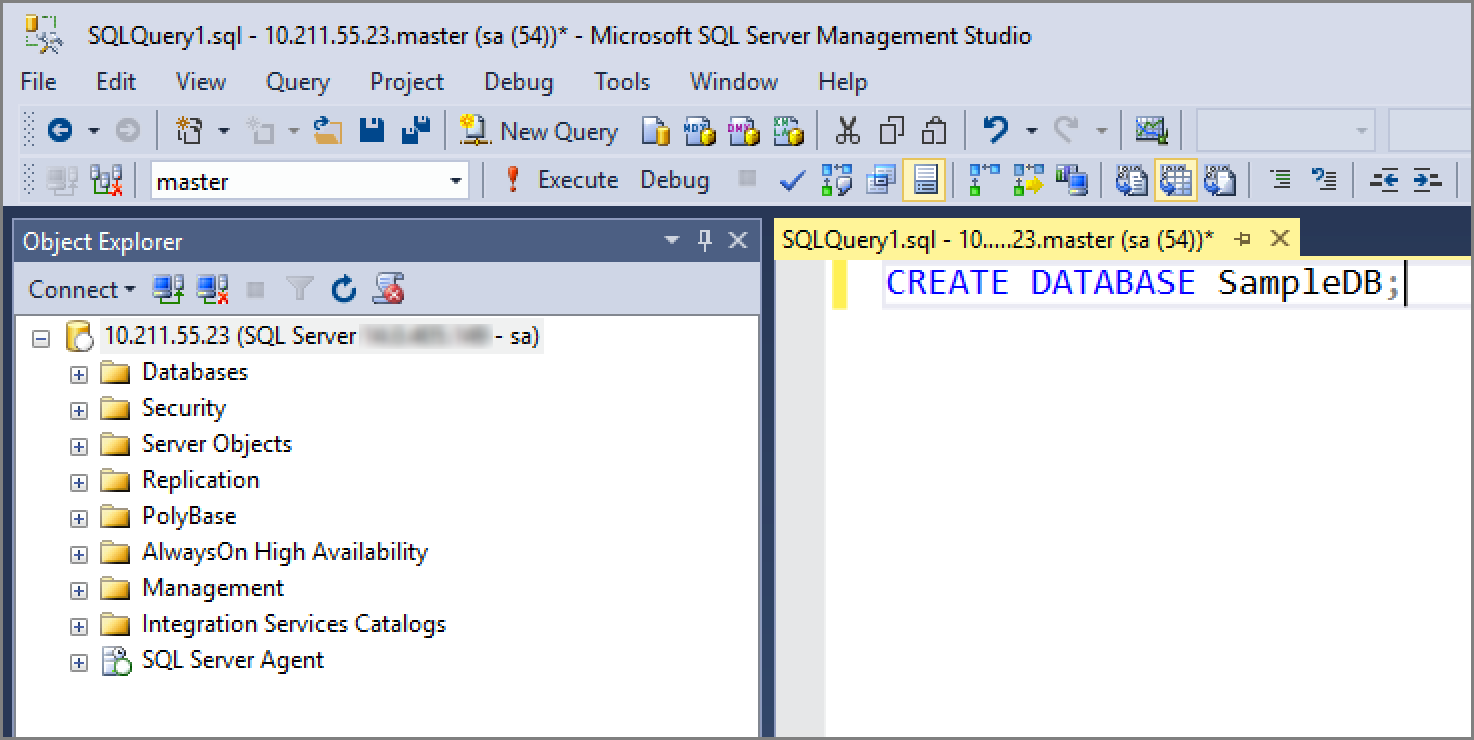
\includegraphics[width=9cm]{./Imagenes/BIimagen8}
\caption{\label{fig:01}Microsoft SQL Server.(Adecuada para realizar un análisis panorámico de la empresa y tomar las mejores decisiones.)}
\end{figure}

\begin{figure}[h!]
\centering

\includegraphics[width=8cm]{./Imagenes/BIimagen9}
\caption{\label{fig:01}JetReports.(Especial para crear informes ERP.)}
\end{figure}

\begin{figure}[h!]
\centering
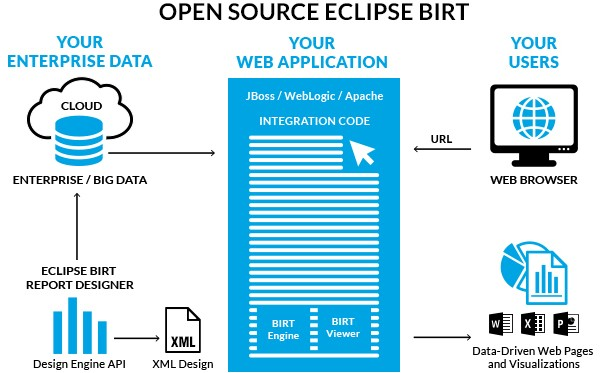
\includegraphics[width=9cm]{./Imagenes/BIimagen10}
\caption{\label{fig:01}Eclipse BIRT Project.(Genera informes para aplicaciones web de código abierto.)}
\end{figure}
\textbf{}\\
\textbf{}\\

\begin{figure}[h!]
\centering
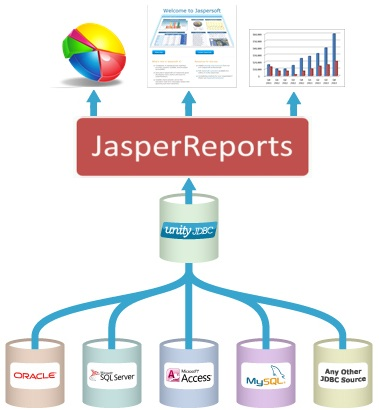
\includegraphics[width=8cm]{./Imagenes/BIimagen11}
\caption{\label{fig:01}JasperReports.(Permite crear informes de rápida impresión.)}
\end{figure}

\begin{figure}[h!]
\centering

\includegraphics[width=5cm]{./Imagenes/BIimagen12}
\caption{\label{fig:01}LogiReport.(Aplicación gratuita basada en web de LogiXML.)}
\end{figure}

\begin{figure}[h!]
\centering
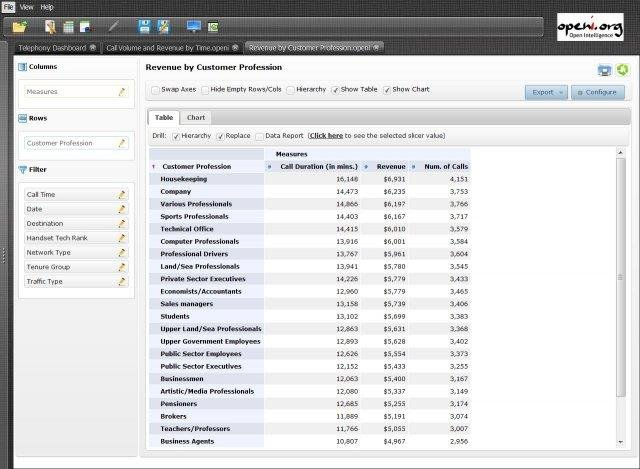
\includegraphics[width=8cm]{./Imagenes/BIimagen13}
\caption{\label{fig:01}OpenI.(Aplicación web orientada al reporting OLAP.)}
\end{figure}

\begin{figure}[h!]
\centering
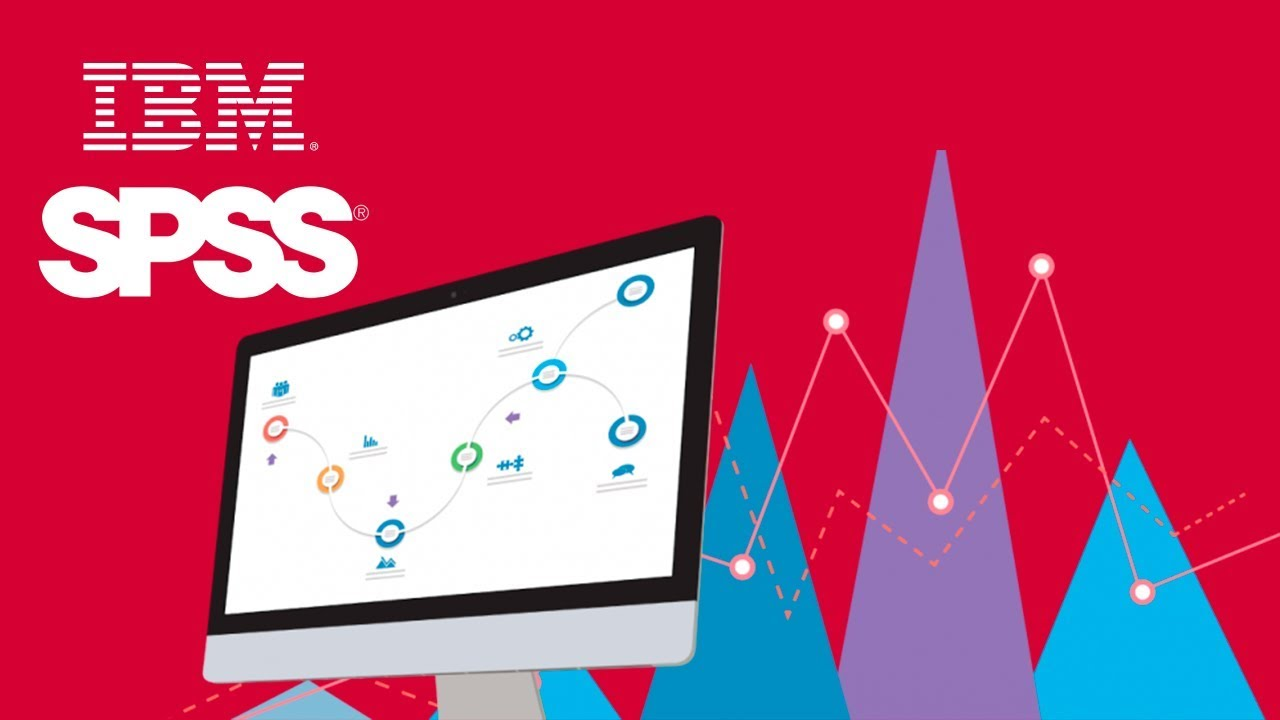
\includegraphics[width=5cm]{./Imagenes/BIimagen14}
\caption{\label{fig:01}SPSS.(Programa estadístico especialmente empleado en ciencias sociales e investigaciones de mercado.)}
\end{figure}

\begin{figure}[h!]
\centering
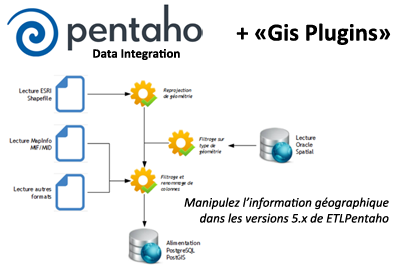
\includegraphics[width=9cm]{./Imagenes/BIimagen15}
\caption{\label{fig:01}Pentaho.(Incluye herramientas para generar informes, minería de datos, ETL, entre otros.)}
\end{figure}

\begin{figure}[h!]
\centering

\includegraphics[width=9cm]{./Imagenes/BIimagen16}
\caption{\label{fig:01}RapidMiner.(Permite analizar datos a través de un entorno gráfico.)}
\end{figure}

\begin{figure}[h!]
\centering
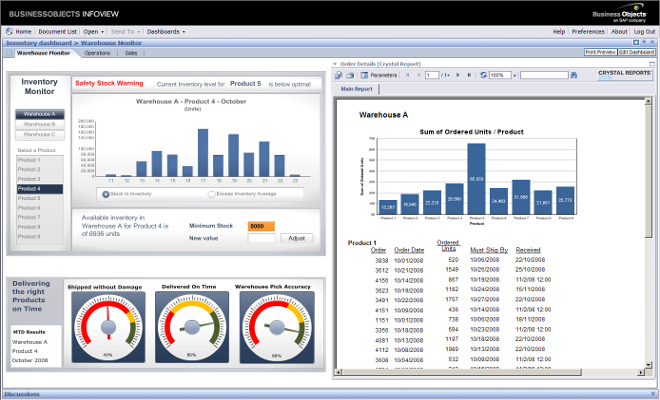
\includegraphics[width=9cm]{./Imagenes/BIimagen17}
\caption{\label{fig:01}Crystal Reports.(Genera informes desde bases de datos múltiples.)}
\end{figure}

\begin{figure}[h!]
\centering

\includegraphics[width=6cm]{./Imagenes/BIimagen18}
\caption{\label{fig:01}ApeSoft.Ofrece una interface sencilla similar a Microsoft Excel.)}
\end{figure}

\begin{figure}[h!]
\centering

\includegraphics[width=6cm]{./Imagenes/BIimagen19}
\caption{\label{fig:01}SAS Institute.(Facilita la gestión de riesgo financiero, desarrollo de modelos de minería de datos, etc.)}
\end{figure}

\begin{figure}[h!]
\centering
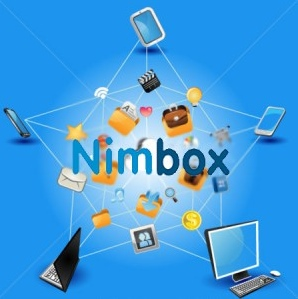
\includegraphics[width=8cm]{./Imagenes/BIimagen20}
\caption{\label{fig:01}NiMbox.(Organiza los datos de la empresa en interactivas aplicaciones.)}
\end{figure}
\textbf{}\\
\textbf{}\\
\section*{3.ANÁLISIS} 
\textbf {3.1 ANÁLISIS (Casos de Uso)}\\
\begin{center}
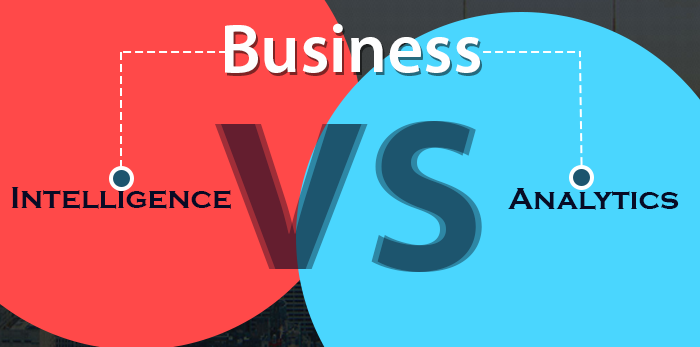
\includegraphics[width=8cm]{./Imagenes/image01}
\end{center}
\begin{center}
\textbf{Business Intelligence vs Business Analytics visto a través del fútbol}\\
\end{center}
Digamos que estás en el cuerpo técnico de un equipo de fútbol y quieres revisar el juego más reciente. Hace esto para ver cómo puede corregir sus errores y replicar sus éxitos.
\item 
Usando nuestras definiciones anteriores,  BI  sería el proceso de identificar todas las estadísticas y jugadas que llevaron a su equipo a ganar. Identificaría que mantuviste la posesión de la pelota por mucho más tiempo que tus oponentes. También identificaría la tendencia de que su lado derecho del campo fue fundamental para retener la posesión a través de pases excelentes.
\item 
El análisis de negocios  estaría más preocupado por la  razón por la  que tuvo posesión de la pelota por más tiempo que su oponente y por qué su lado derecho del campo le fue tan bien al pasar.

\subsubsection*{Fue porque:}\\
\item - ¿Los defensores de tu oponente en ese lado eran jugadores más débiles que sus defensores en el otro?
\item - ¿Tus jugadores del lado derecho habían estado pasando más tiempo juntos en el campo que tu lado izquierdo?
\item - ¿Uno de tus jugadores de la derecha simplemente tenía un rendimiento fenomenal que se trasladó al resto de ese lado?

\item 
Estas preguntas son importantes. Le permiten descubrir cómo puede replicar su éxito o prevenir su fracaso en el futuro. Hacer las preguntas  correctas de inteligencia empresarial  lo llevará a mejores análisis. Al usar un tablero de negocios , todas las ideas se pueden simplificar en un solo lugar, haciendo que el tiempo para tomar decisiones significativas sea mucho más rápido. Pero primero, necesitamos analizar más la diferencia, ya que eso nos ayudará a comprender qué hacer en el proceso de operación de una empresa y cómo elegir la mejor herramienta para administrar sus conocimientos.
\item 
\item 
\textbf{¿Cómo se aplica esto a los negocios?}\\
\item 
¿Puede comprender los factores que están  causando  el éxito o el fracaso de su negocio en lugar de solo los factores  asociados  con el éxito o el fracaso de su negocio? Si es así, es mucho más probable que pueda predecir el futuro en su mercado y actuar en consecuencia. Sin embargo, es importante tener en cuenta que necesita saber qué está correlacionado con algo antes de poder conocer la causalidad.
\item
En otras palabras, debe saber  qué  sucedió y  cómo  sucedió (BI) antes de poder decir  por qué  sucedieron las cosas (BA) con un grado razonable de certeza.
\item
\item
\textbf{Escenarios de casos de uso}\\
\item
Solidifiquemos las cosas y terminemos esta publicación con ejemplos de negocios, ilustrando la diferencia entre inteligencia empresarial y análisis de negocios.
\item
Supongamos que trabaja para una empresa de marketing que utiliza inteligencia empresarial y análisis para ayudar a las grandes empresas de comercio electrónico a lanzar nuevos productos. Para comprender qué productos nuevos tendrían más probabilidades de tener éxito (análisis), necesitaría descubrir:
\item 
- Qué productos han tenido más éxito en el pasado (BI)
\item 
- Las tendencias estacionales que han influido en el éxito de lanzamientos anteriores (BI)
\item 
- Por qué los clientes compraron los productos exitosos del pasado (BA)
\textbf{}\\
\textbf{}\\
\textbf{¿Qué diferencia existe entre el Business Intelligence y el Business Analytics?}\\
\textbf{}\\
\textbf{Una mirada al pasado:}\\
\textbf{}\\
Business Intelligence (BI) permite visualizar y hacer análisis con base en la información histórica y es fundamental para que las empresas tomen decisiones, pues brinda un panorama de cómo se ha desarrollado históricamente un negocio. BI es también una categoría de aplicaciones y tecnologías para la recolección, almacenamiento, análisis y acceso a los datos para ayudar a los usuarios empresariales a tomar menores decisiones de negocios.
\item
\textbf{La mirada al futuro:}\\
\textbf{}\\
Por su parte, Business Analytics (BA) se encarga de visualizar el futuro con base en la experiencia y la información y modelos predictivos que se conocen del negocio para anticiparse a las decisiones y
mejorar la competitividad. Es la practica de la explotación iterativa y metódica de datos de una organización con énfasis en el análisis estadístico y se utiliza para automatizar y optimizar los procesos de negocio.
\item
\textbf{La gran  diferencia que existe entre el BI y BA, es que el Business Intelligence mira  hacia el pasado permitiendo visualizar y hacer analisis con base  en la información histórica para  ayudar a los usuarios empresariales a tomar menores decisiones de negocios, y el Business Analytics da una mirada hacia el futuro para  prevenir futuros problemas que puedan ocurrir en la empresa en  base  a la  experiencia e información  que  se  conocen del  negocio  para anticiparse a las decisiones y mejorar la competitividad.}

\item
\begin{center}
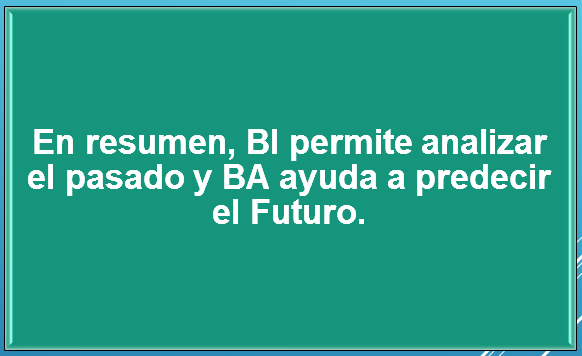
\includegraphics[width=10cm]{./Imagenes/image05}
\end{center}
\item

\begin{center}
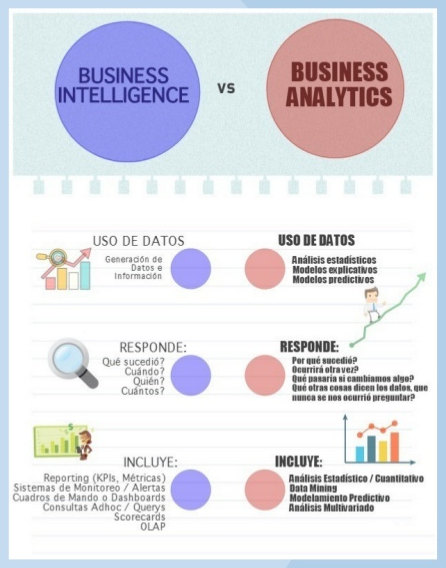
\includegraphics[width=10cm]{./Imagenes/image02}
\end{center}
\subsubsection*{CONCLUSIONES} 

\item En forma exclusiva, la inteligencia empresarial y el análisis de negocios forman los componentes esenciales requeridos por una empresa para administrar su información de manera efectiva.
\textbf{}\\
\item 
Las dos terminologías parecen tener similitudes de una manera que hace que los estudiantes deduzcan que están conectados. De hecho, vale la pena reconocer que la analítica es una función de la inteligencia empresarial. La información analizada mediante análisis para predecir el futuro es la misma información obtenida del componente de inteligencia de la empresa. Tanto BI como BA se enfocan en impulsar a la compañía a avanzar enérgicamente.
\textbf{}\\
\item En un medio globalizado y audaz como el del mundo empresarial, podemos ver que el entorno en el que la inmensa mayoría de las empresas tiene soportados los procesos de negocio con diferentes sistemas de información y estrategias, los ubica en un mercado tan competitivo como el actual, Hoy se ha convertido en un problema, por lo que la Inteligencia de Negocios se erige como una pieza clave para ser proactivo a la hora de tomar mejores decisiones y de conseguir mejor control de negocio y ventajas que nos diferencien de la competencia.
\textbf{}\\
\item Lo que HEMOS APRENDIDO es que la gran mayoría de empresas no utilizan sistemas de inteligencia empresarial para gestionar sus negocios. Sin embargo, SABEMOS QUE SI ENTIENDEN EL CONCEPTO, y saben que son herramientas muy enriquecedoras para la gestión actual, a lo que añaden las siguientes ventajas para el  uso de Software de Inteligencia de Negocios: 
\textbf{}\\
\textbf{}\\
– Los sistemas de Business Intelligence ayudan a hacer más competitiva la estrategia de la empresa.\textbf{}\\

– Apoyan la toma de decisiones que son vitales para obtener mejores resultados.\textbf{}\\

– La Inteligencia de Negocios facilita notablemente la interactividad entre usuarios, clientes y proveedores.\textbf{}\\

– Facilitan el acceso a los datos críticos de la empresa y las informaciones corporativas para la integración de datos y la toma de decisiones.\textbf{}\\

– Permite alinear acciones de diferentes departamentos e igualmente ayuda a controlar cada línea de negocio o departamento con métricas específicas.\textbf{}\\
\textbf{}\\

\newpage\subsection*{Sitios Web Relacionados}
\begin{enumerate}
\item http://revistas.utp.edu.co/index.php/revist-aciencia/article/view/1803/1209
\item https://www.sciencedirect.com/science/arti-cle/pii/S0186104215000807
\item http://www.spentamexico.org/v4-n2/4(2)\%2016-52.pdf
\item https://selecthub.com/business-intelligence/business-intelligence-vs-business-analytics
\item https://www.betterbuys.com/bi/business-intelligence-vs-business-analytics
\item https://aprendebi.wordpress.com/2016/11/3-0/bussiness-intelligence-vs-bussiness-analytics
\item http://scholarium.info/analisis-de-negocio-business-analysis-ba
\item https://blog.corponet.com.mx/que-es-la-inteligencia-de-negocios
\item http://www.emb.cl/gerencia/articulo.mvc?xi-d=1769&sec=9
\item https://softwareyhardware.com/software/busi-ness-intelligence-vs-business-analytics-diferencias/
\end{enumerate}


\end{document}
